\documentclass[11pt]{article}
\usepackage[leqno]{amsmath}
\usepackage{amssymb}
\usepackage{color}
%\usepackage{leqno}
\usepackage{ulem}
\usepackage{indentfirst}
\usepackage{natbib}
\usepackage{amsthm}
\usepackage{ragged2e}
\usepackage{graphicx}
%\usepackage{setspace}
%\doublespacing
%\usepackage{enumitem}
\usepackage[compatibility=false]{caption}
\textwidth 6.5in
\textheight 9in
\topmargin -0.5in
\setcitestyle{square}
\oddsidemargin 0.00in
\evensidemargin 0.00in

\renewcommand{\baselinestretch}{1.2}

\setcounter{page}{1}
\usepackage[figurewithin=section]{caption}


\begin{document}
	\begin{center}
		\textbf{\large Review of Generalized Alternating Minimization Framework for Convergence of Incremental EM and Variational EM Algorithms}\\
		{Huyen Nguyen$^1$ \\
			$^1$Department of Statistics, University of Connecticut, Storrs, CT, 06269}
	\end{center}
	\begin{abstract}
		The expectation-maximization (EM) algorithm is a well-known computational method to obtain the maximum likelihood estimator for the incomplete data problem. The algorithm consists of two steps: the first step is to compute the expectation of the likelihood function, i.e the E-step, and the second step is to maximize this expectation, i.e the M-step. 
	\end{abstract}
	
	\noindent
	Keywords: expectation maximization, Monte Carlo methods, importance sampling, Robbin-Monro algorithm, non-linear mixed effects model
	\section{Introduction}
	Expectation Maximization (EM) is a popular algorithm to compute the maximum likelihood estimator in missing data problems. We assume that the complete data consists of $(X, Z)$ with only $X$ being observed. Let $\ell(\theta; X, Z)$ denote the complete-data log likelihood, in which $\theta$ is the unknown parameter vector that we wish to obtain the maximum likelihood estimate of. In other words, given an outcome of $(X, Z)$, we maximize the log likelihood function with respect to $\theta$ over its parameter space. The EM algorithm is an iterative method to compute the estimate.
	\begin{itemize}
		\item \textbf{E step:} In the E step, we compute the log likelihood of the complete data $\ell(\theta; X, Z)$ given the observed data $X$ and current parameter estimate $\theta_t$
		\begin{equation}
			\label{expectation}
			Q(\theta \vert \theta_t) = E [\ell(\theta; X, Z) \vert X, \theta_t]
		\end{equation}
		\item \textbf{M step:} In the M step, we maximize $Q(\theta_{t+1} \vert \theta_t)$ over $\theta$ 
		\begin{equation}
			\theta_{t+1} = \arg \max_\theta Q(\theta \vert \theta_t)
		\end{equation}
	\end{itemize}
	The maximum likelihood estimate of $\theta$ is then the best of local maximums obtained by iterations of the EM algorithm. To show why the EM algorithm works, we can use the Jensen's inequality by the concavity of the natural logarithm function (\cite{roche2011algorithm}). Let $p(\cdot \vert \cdot)$ denote the general conditional probability density function.
	\begin{equation}
		\label{yitworks}
		\begin{split}
			\ell(\theta; X) - \ell (\theta_t; X)
			& = \ln \frac{p(x\vert \theta)}{p( x \vert \theta_t) } \\
			& = \ln \int \frac{p(x, z\vert \theta)}{p( x \vert \theta_t)} dz\\
			& = \ln \int \frac{p(x, z\vert \theta)}{p( x,z \vert \theta_t)} p(z \vert x, \theta_t) dz \\
			& \geq \int \ln \frac{p(x, z\vert \theta)}{p( x,z \vert \theta_t)} p(z \vert x, \theta_t) dz \\
			& = Q(\theta \vert \theta_t) - Q(\theta_t \vert \theta_t)
		\end{split}
	\end{equation}
	Thus, (\ref{yitworks}) shows that any value of $\theta$ that increases $Q(\theta \vert \theta_t)$ in (\ref{expectation}) beyond $Q(\theta_t \vert \theta_t)$ will also increase $\ell(\theta; X)$ beyond $\ell(\theta_t; X)$ (\cite{roche2011algorithm}). There are numerous variants of the EM algorithm to adapt to practical applications. One of the issues commonly encountered is the intractability of the expectation in the E-step and an approximation method is needed to approximate the expectation. 
	
	In their paper, \cite{gunawardana2005convergence} introduced the generalized alternating minimization (GAM) framework and derive convergence results for variants of EM algorithm.
	
	In section \ref{gam}, we introduce the generalized alternating  minimization framework introduced by this paper and their convergence theorem result. Section \ref{incremental} and \ref{variational} present the results of GAM framework on the incremental EM Algorithm and the variational EM Algorithm, respectively.
	
	\section{Convergence Results of the GAM Framework} \label{gam}
	In this section, we introduce the generalized alternating  minimization framework introduced by this paper and their convergence theorem result.
	Fig (\ref{fig:examplefig}) shows an example of a figure.
	
	\begin{figure}[!ht]
		\label{fig:examplefig}
		\centering
		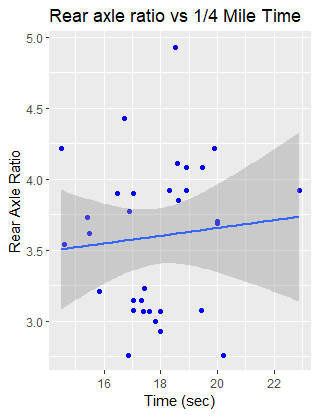
\includegraphics{examplefig.png}
		\caption{Scatterplot of Rear Axle versus Time (in seconds)}
	\end{figure}
	
	\section{Incremental EM Algorithm} \label{incremental}
	In this section, we present the results of GAM framework on the incremental EM Algorithm. 
	\section{Variational EM Algorithm} \label{variational}
	In this section, we present the result of the GAM framework on the variational EM algorithm.
	Table (\ref{tab:exampletab}) shows an example of a table in latex
	\begin{table}[!ht]
		\centering
		\begin{tabular}{|c|c|c|c|c|c|}
			\hline
			Gear & Cyl = 4 & Cyl = 6 & Cyl = 8\\
			\hline
			3 & 1 &  2 & 12 \\
			4 & 8 & 4  & 0 \\
			5 & 2 & 1 & 2 \\
			\hline
		\end{tabular}
		\caption{This is an example of a table}
		\label{tab:exampletab}
	\end{table}
	\section*{Appendix}
	This is the Appendix section.
	
	\bibliographystyle{apalike}
    \bibliography{projectrefs}
\end{document}
